\subsection{Area operatore}
Dopo aver cliccato il pulsante \emph{Gestisci area operatore} nella schermata Home, verrà visualizzata la schermata di accesso e registrazione per gli operatori:
\begin{figure}[H]
    \centering
    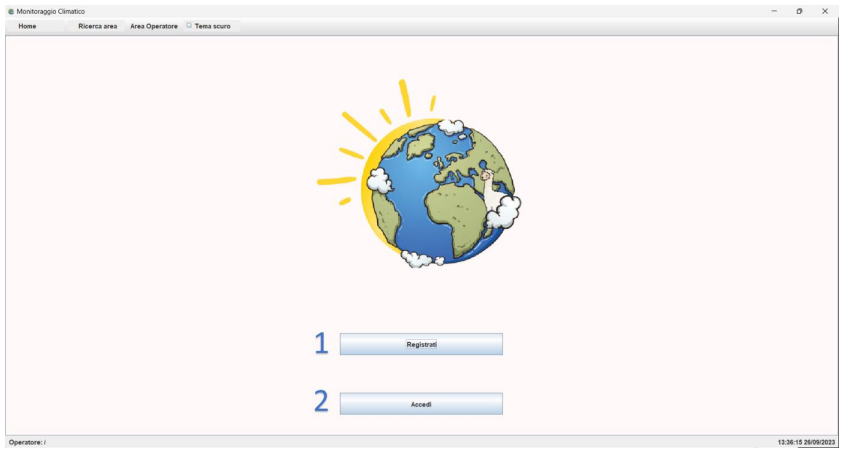
\includegraphics[width=1\textwidth]{../../img/schermata_area_operatore.png}
    \caption{Schermata Area operatore}
\end{figure}

Il pulsante \emph{Registrati} permette di accedere alla schermata di registrazione:
\begin{figure}[H]
    \centering
    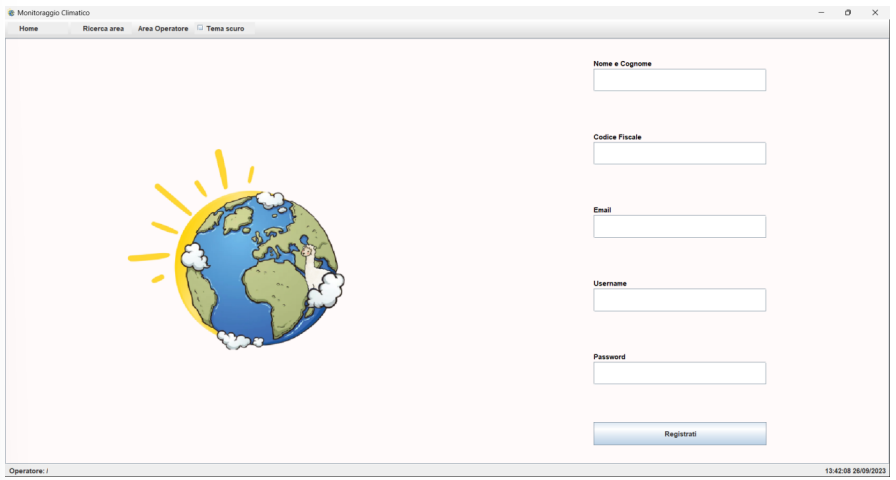
\includegraphics[width=1\textwidth]{../../img/schermata_registrazione.png}
    \caption{Schermata Registrazione}
\end{figure}

Qui è possibile inserire i propri dati personali e scegliere un nome utente e una password per accedere all'applicazione:
\begin{itemize}
    \item Nome e Cognome (Es. Mario Rossi).
    \item Codice fiscale (Es. RSSMRA01A01H501A).
    \item E-mail (Es. mario.rossi@gmail.com).
    \item Username (Es. MarioRossi).
    \item Password (Es. MarioRossi00!).
\end{itemize}

Una volta inseriti correttamente i dati, cliccare il pulsante \emph{Registrati} per completare la registrazione.

Dopo aver effettuato la registrazione, è possibile effettuare l'accesso inserendo il proprio username e la propria password nella schermata di accesso:
\begin{figure}[H]
    \centering
    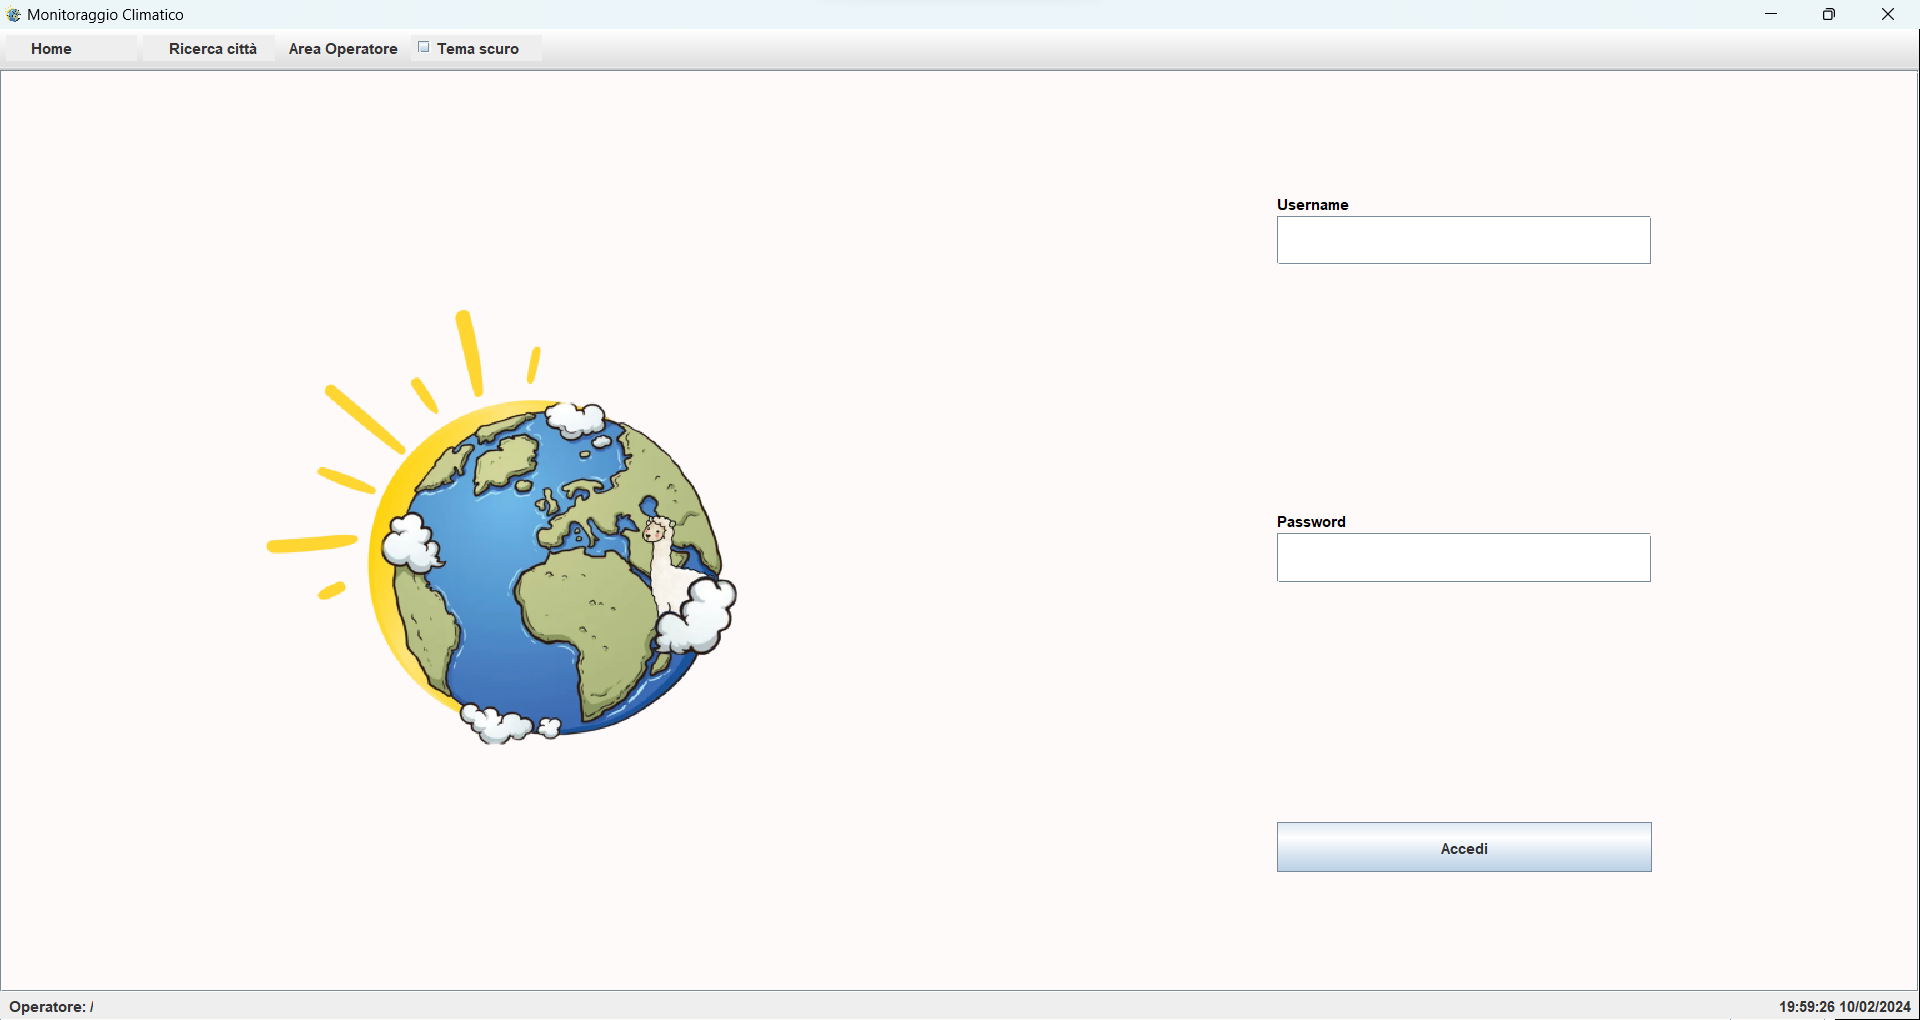
\includegraphics[width=1\textwidth]{../../img/schermata_login.png}
    \caption{Schermata Accesso}
\end{figure}

Una volta effettuato l'accesso, apparirà la seguente finestra: 
\begin{figure}[H]
    \centering
    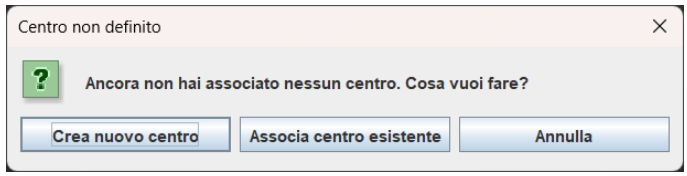
\includegraphics[width=1\textwidth]{../../img/finestra_centro.png}
    \caption{Finestra di dialogo Centro}
\end{figure}

Se si clicca \emph{Associa centro esistente} vengono viasualizzati, se presenti, i centri di monitoraggio nel sistema:
\begin{figure}[H]
    \centering
    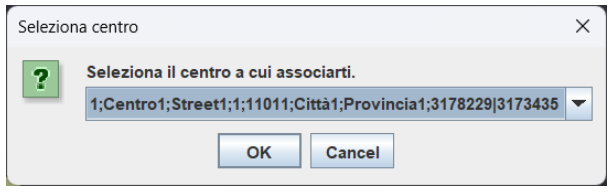
\includegraphics[width=1\textwidth]{../../img/seleziona_centro.png}
    \caption{Finestra di dialogo per la selezione del centro}
\end{figure}

Se il centro a cui ci si vuole associare non è presentare, cliccando \emph{Cancel} si torna alla finestra precedente e si può procedere a creare il prorpio
centro di monitoraggio inserendo i dati relativi ad esso:
\begin{figure}[H]
    \centering
    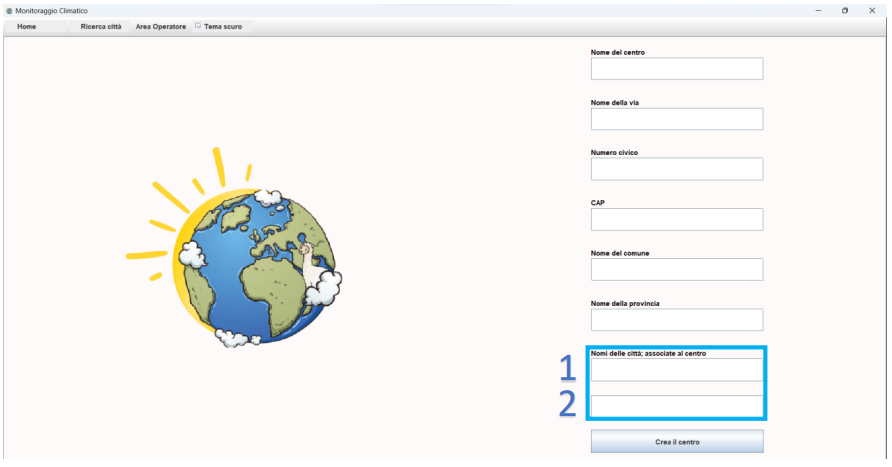
\includegraphics[width=1\textwidth]{../../img/schermata_creazione_centro.png}
    \caption{Schermata Creazione centro}
\end{figure}

Per inserire correttamente il nome delle città, si scrive il suo nome nel campo [1] e si preme il pulsante \emph{Invio}; se sono presenti più città
con lo stesso nome,
sarà possibile specificare quale aggiungere scegliendo dal menù che appare: 
\begin{figure}[H]
    \centering
    \includegraphics[width=1\textwidth]{../../img/scelta_città.png}
    \caption{Finestra per la scelta della città}
\end{figure}

Una volta selezionata la città desiderata, comparirà nel campo [2] con i sui dati geografici associati:
\begin{figure}[H]
    \centering
    \includegraphics[width=0.7\textwidth]{../../img/esempio_città_associata.png}
    \caption{Esempio città associata correttamente}
\end{figure}

Questo procedimento si ripete per ogni città che si vuole associare al centro di monitoraggio.\\
Se si sbaglia ad inserire una città, è possibile rimuoverla cliccando sul suo nome nel campo [2] ed eliminandola:
\begin{figure}[H]
    \centering
    \includegraphics[width=1\textwidth]{../../img/esempio_città_eliminata.png}
    \caption{Esempio città rimossa correttamente}
\end{figure}

\textcolor{red}{ATTENZIONE:} una volta creato un centro di monitoraggio, non è possibile modificare i dati inseriti o eliminarlo.\\